\documentclass{beamer}

\usepackage[utf8]{inputenc}
\usepackage{lmodern} 
\usepackage[utf8]{inputenc}
\usepackage{lmodern} 
\usepackage{listings}
\usepackage{xcolor} 
\usepackage{graphicx}
\definecolor{myblue}{RGB}{48, 63, 159}
\setbeamercolor{palette primary}{bg=myblue, fg=white}
\setbeamercolor{structure}{fg=myblue}
\setbeamercolor{frametitle}{bg=myblue, fg=white}
\setbeamercolor{title}{bg=myblue, fg=white}
\setbeamercolor{footlinecolor}{bg=myblue, fg=white}


\defbeamertemplate*{title page}{mytemplate}{
	\vfill
	\begin{center}

		\begin{beamercolorbox}[wd=0.8\paperwidth, center, rounded=true, shadow=true]{title}
			\usebeamerfont{title}\inserttitle\par
		\end{beamercolorbox}
		\vspace{2cm} 

		\usebeamerfont{author}\insertauthor
		\vspace{1cm} 
		\usebeamerfont{date}\insertdate
	\end{center}
	\vfill
}


\defbeamertemplate*{frametitle}{mytemplate}{
	\begin{beamercolorbox}[wd=\paperwidth, ht=2.5ex, dp=1.5ex, left]{frametitle}
		\hspace{1em}\usebeamerfont{frametitle}\insertframetitle
	\end{beamercolorbox}
}


\setbeamertemplate{footline}{
	\begin{beamercolorbox}[wd=\paperwidth, ht=2.25ex, dp=1ex]{footlinecolor}
		\hspace{1em}\usebeamerfont{author in footline}\insertshortauthor
		\hfill
		\usebeamerfont{title in footline}\insertshorttitle
		\hfill
		\usebeamerfont{date in footline}\insertdate \hspace{1em} \insertframenumber/\inserttotalframenumber \hspace{0.5em}
	\end{beamercolorbox}
}


\setbeamerfont{author in footline}{size=\tiny}
\setbeamerfont{title in footline}{size=\tiny}
\setbeamerfont{date in footline}{size=\tiny}

\newcommand{\myvec}[1]{\ensuremath{\begin{pmatrix}#1\end{pmatrix}}}
\providecommand{\brak}[1]{\ensuremath{\left(#1\right)}}


\title{4.7.50}
\author{Shriyansh Chawda-EE25BTECH11052}
\date{August 23, 2025}



\begin{document}
	

		\setbeamertemplate{footline}{} 
		\frame{\titlepage}
	
\begin{frame}{Question} 
	Find the vector equation of the line passing through (1, 2, 3) and perpendicular to the $\vec{r}\cdot(\hat{i} + 2\hat{j} - 5\hat{k}) + 9 = 0$.
	\end{frame}
	
\begin{frame}{Solution}
The plane is given by
\begin{equation}
	\mathbf r \cdot \brak{1, 2, -5} + 9 = 0
\end{equation}
so the plane's normal vector is
\begin{equation}
	\mathbf n = \myvec{1 \\ 2 \\ -5}.
\end{equation}
The required line is perpendicular to the plane, so its direction vector lies in the row space. Thus, the line direction vector can be chosen as
\begin{equation}
	\mathbf d = \mathbf n = \myvec{1 \\ 2 \\ -5}.
\end{equation}
\end{frame}

\begin{frame}{Solution}
Using the point
\begin{equation}
	\mathbf a = \myvec{1 \\ 2 \\ 3},
\end{equation}
the vector equation of the line is
\begin{equation}
	\mathbf r = \mathbf a + t\mathbf d
\end{equation}
\begin{equation}
	\mathbf r = \myvec{1 \\ 2 \\ 3} + t \myvec{1 \\ 2 \\ -5}, \quad t \in \mathbb R.
\end{equation}
In symmetric form, the line is
\begin{equation}
	\frac{x-1}{1} = \frac{y-2}{2} = \frac{z-3}{-5}.
\end{equation}
\end{frame}

\begin{frame}{Plot}
\begin{figure}[H]
	\centering
	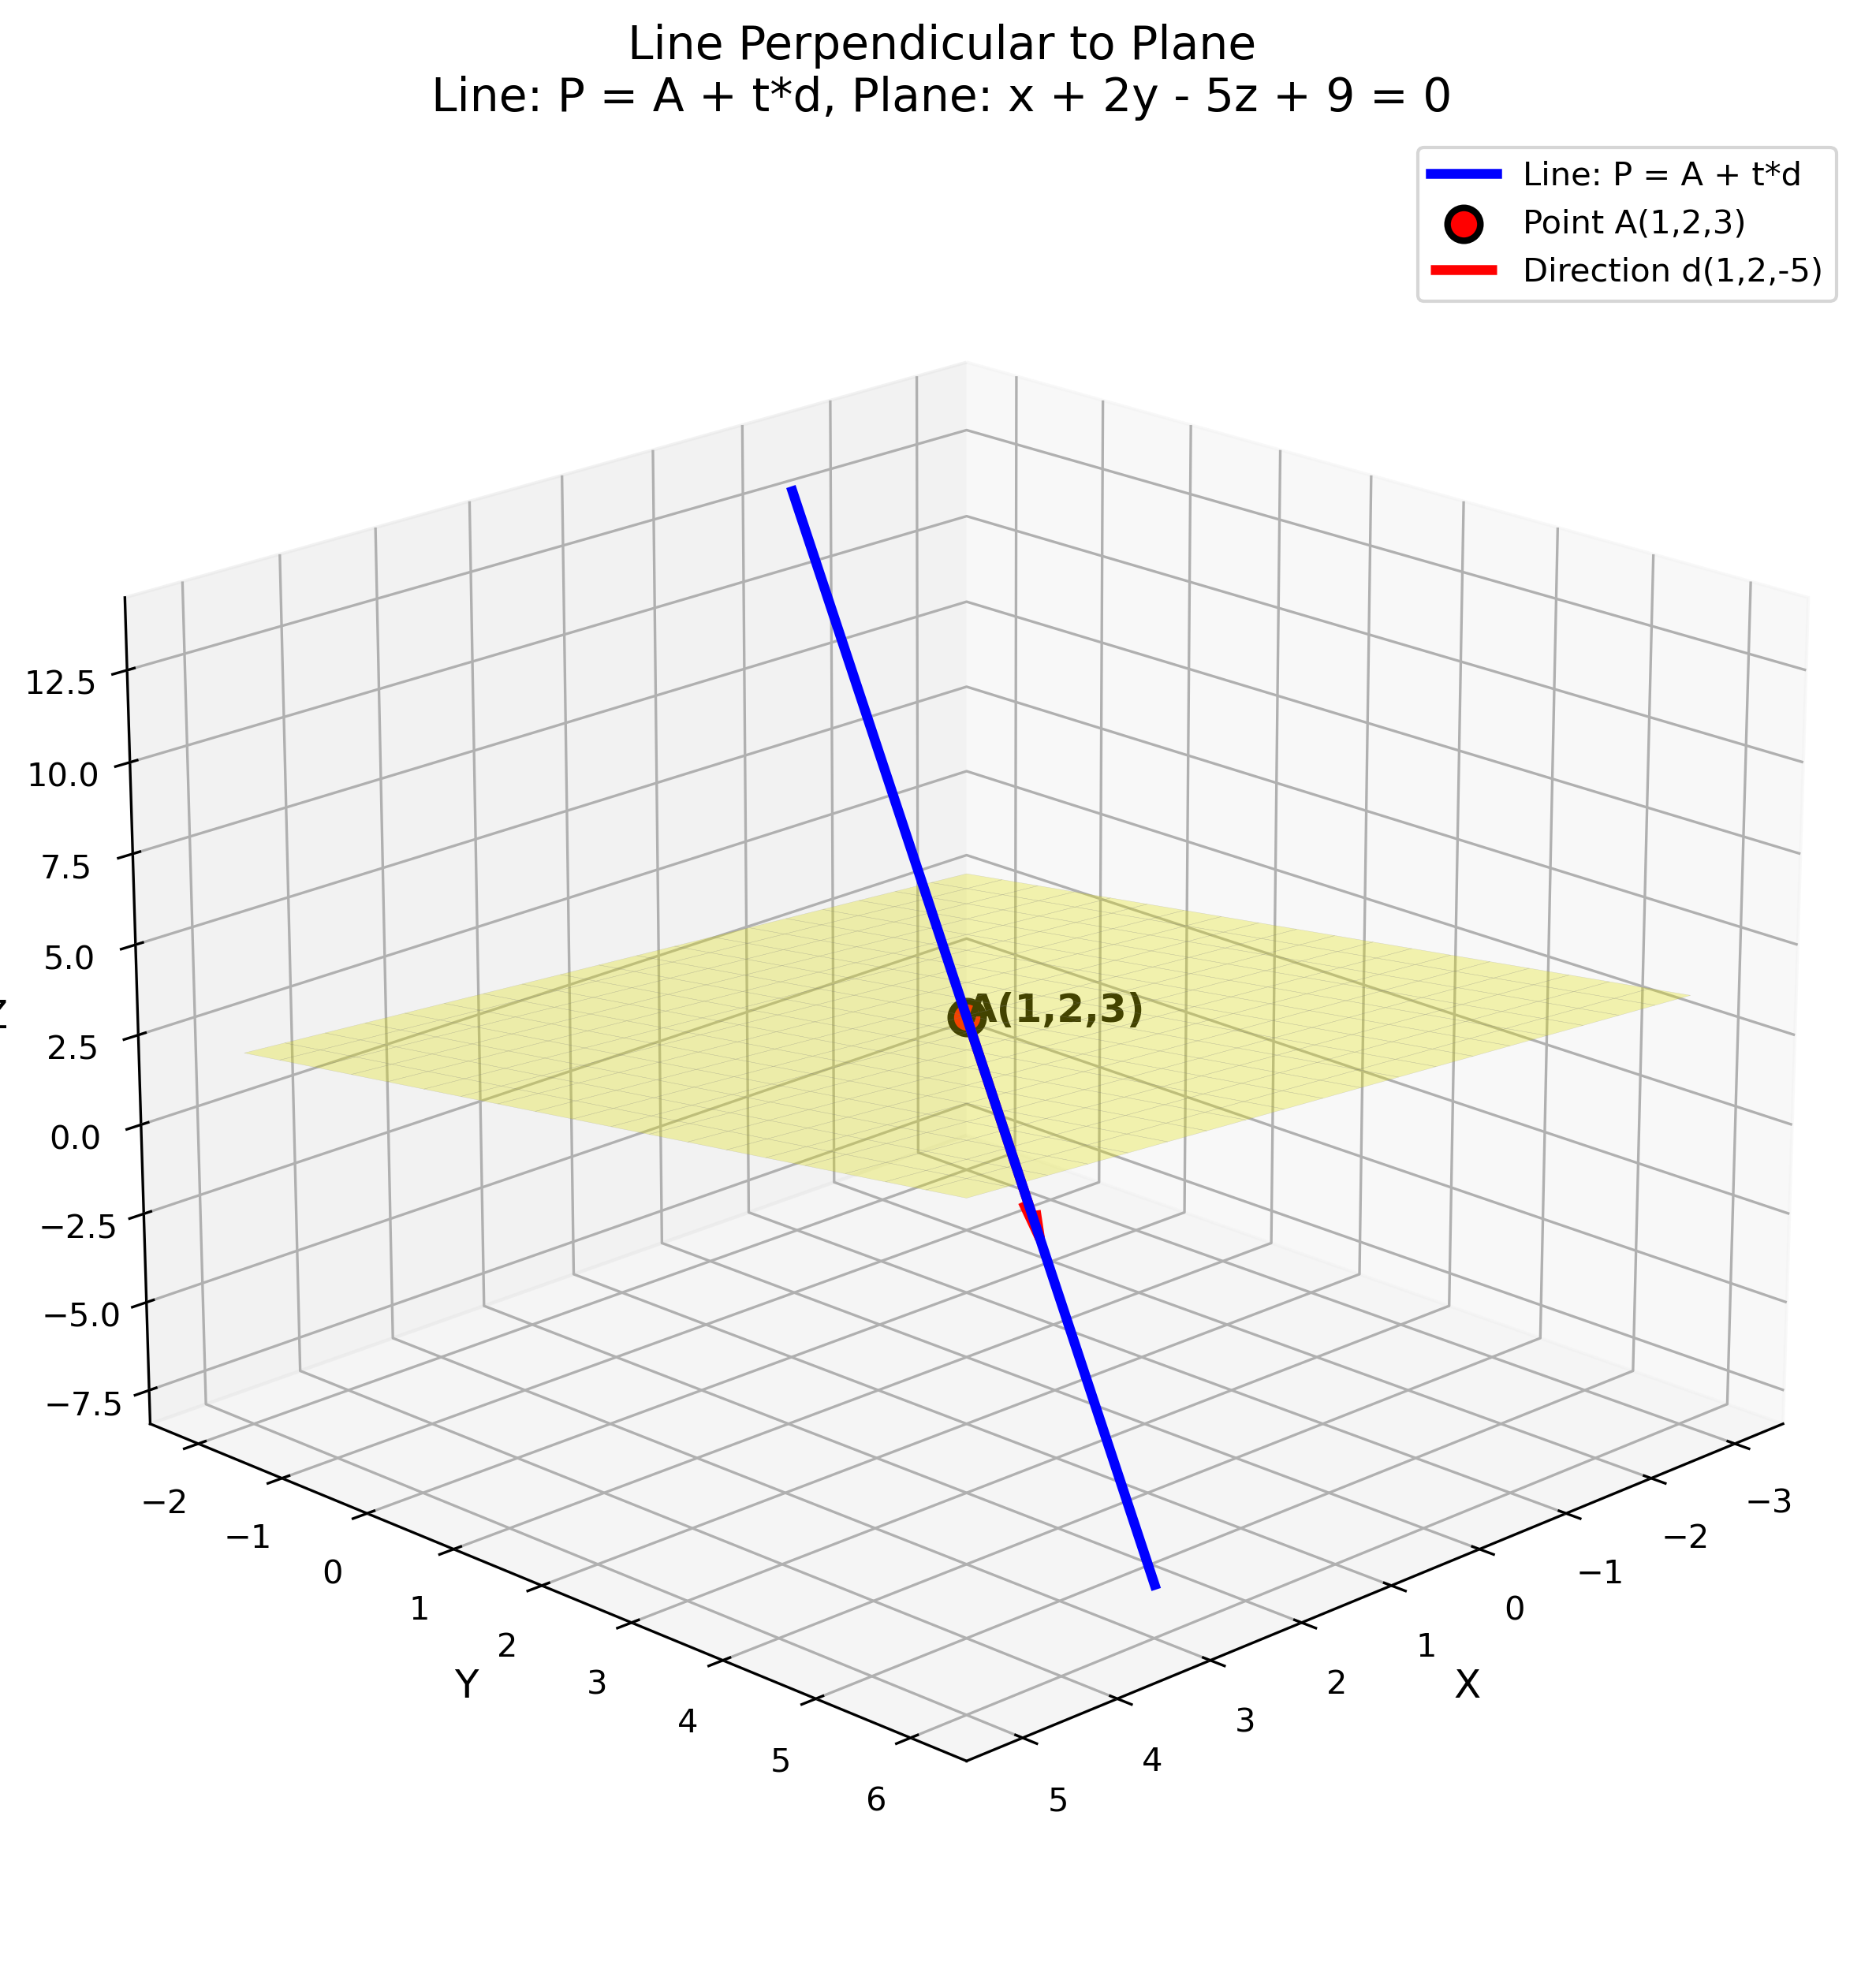
\includegraphics[width=0.8\linewidth]{figs/line_perpendicular}
	\caption{}
	\label{fig:lineperpendicular}
\end{figure}

\end{frame}





\end{document}